\documentclass[a4paper,oneside,11pt]{article}
\usepackage[utf8]{inputenc}
\usepackage[T1]{fontenc}
\usepackage[brazil]{babel}
\usepackage{graphicx,amsmath,amssymb,booktabs,longtable,array,float}
\usepackage[a4paper,left=2.5cm,right=2cm,top=3cm,bottom=2.5cm]{geometry}
\usepackage{fancyhdr,setspace,microtype}
\usepackage[hidelinks]{hyperref}
\setlength{\headheight}{32pt}
\pagestyle{fancy}\fancyhf{}
\lhead{
\includegraphics[height=0.9cm]{figuras/ufc.pdf}}
\chead{\small CNN para localização de linha}\rfoot{\thepage}
\onehalfspacing
\newcommand{\autores}{Preencher nomes dos autores}
\newcommand{\disciplina}{Preencher disciplina}
\begin{document}
\begin{titlepage}\centering

\includegraphics[width=0.12\textwidth]{figuras/ufc.pdf}\\[0.5cm]
{\bfseries\large UNIVERSIDADE FEDERAL DO CEARÁ\\ CAMPUS JARDINS DE ANITA -- ITAPAJÉ}\\[2.5cm]
{\bfseries\LARGE Localização de linha com rede neural convolucional: construção do dataset e avaliação offline em frames de vídeos}\\[2cm]
{\large\textbf{Autores:} \autores}\\[1cm]
{\large\textbf{Disciplina:} \disciplina}
\vfill Itapajé, novembro de 2026
\end{titlepage}
\tableofcontents\newpage
\section*{Resumo do Projeto}\addcontentsline{toc}{section}{Resumo do Projeto}
Este relatório descreve a preparação e a avaliação de uma rede neural convolucional (CNN) para localizar horizontalmente a linha de uma pista a partir de imagens extraídas de vídeos. O trabalho compreendeu a análise inicial de segmentação, a criação de marcações humanas, o auxílio à rotulagem com OpenCV e dois experimentos supervisionados com a mesma arquitetura implementada em NumPy. O acervo contém 1.032 frames de nove vídeos; no segundo experimento, 87 imagens foram revisadas e 77 utilizadas. O treino aumentou de 24 para 58 imagens, mantendo dez imagens de validação e nove de teste. O erro absoluto médio de teste caiu de 0,1373 para 0,0725 na coordenada normalizada, aproximadamente de 6,9\% para 3,6\% da largura. Os resultados são exploratórios: o teste já havia sido consultado e a amostra é pequena. A avaliação ocorreu exclusivamente offline, sem câmera ao vivo, acionamento de motores ou comprovação de seguimento autônomo da pista.

\section{Introdução e objetivos}
O robô seguidor de linha precisa identificar a trajetória apesar de sombras, variações de exposição, rejuntes e descontinuidades da fita. Uma estratégia baseada apenas em regiões escuras pode confundir a pista com elementos do piso. O objetivo desta etapa foi investigar se uma CNN pequena consegue aprender a posição da linha usando exemplos revisados por uma pessoa.

A tarefa efetivamente treinada é uma regressão: dada uma imagem, estimar a coordenada horizontal da trajetória na altura de referência de 75\% da imagem original. Uma posição negativa indica a região à esquerda; positiva, à direita. Essa coordenada não é um comando de motor, uma velocidade ou um ângulo de direção. A transformação da percepção em controle permanece uma etapa futura.

O escopo documentado é o dos artefatos preservados no projeto: dois treinos, suas métricas, rótulos, previsões e gráficos. Não houve nova execução de treinamento para produzir este relatório. Não há avaliação com câmera em tempo real nem demonstração de deslocamento físico do robô associada a esses resultados.

\section{Construção do dataset}
\subsection{Acervo e rastreabilidade}
Foram reunidos 1.032 arquivos JPG de nove vídeos. Os metadados associam cada imagem ao vídeo de origem, timestamp e resolução. Os registros observados usam imagens de 1.080 por 1.920 pixels e timestamps espaçados em 0,5 segundo. O número de frames existentes não corresponde ao número de exemplos supervisionados: uma imagem só pode entrar na regressão quando possui marcação válida na altura de referência.

O estudo inicial selecionou cinco frames por vídeo, totalizando 45 amostras. Foram examinadas 1.215 combinações de limiarização, morfologia e região de interesse. Essa análise serviu para entender falhas de segmentação; suas medidas de máscara não representam acurácia da CNN. Cruzamentos, rejuntes e alterações de iluminação mostraram que escolher o maior componente escuro pode deslocar a trajetória estimada.

\subsection{Marcação humana e critérios de inclusão}
A trajetória foi representada por pontos em coordenadas da imagem original. A posição horizontal de referência é interpolada entre pontos humanos que abrangem a altura escolhida. Não se extrapola a trajetória para regiões sem anotação. Imagens parciais podem participar se os pontos cobrirem essa referência; estados ausente e ambíguo ficam fora da regressão.

No primeiro experimento, 45 imagens foram revisadas, 43 aproveitadas e duas excluídas. No segundo, 87 imagens únicas foram revisadas, das quais 77 aproveitadas. Das dez excluídas, sete não cobrem a referência, duas são ambíguas e uma está marcada como ausente. Foram acrescentadas 42 revisões, todas do primeiro vídeo, gerando 34 exemplos utilizáveis adicionais de treino. Assim, 39 dos 58 exemplos de treino vêm desse único vídeo, o que concentra a distribuição e limita a diversidade.

\subsection{Separação por vídeo}
Os conjuntos foram separados por vídeo de origem para evitar que frames próximos de uma mesma gravação aparecessem em treino e teste. As dez imagens de validação e as nove de teste, com os mesmos alvos e tensores de entrada, foram preservadas nos dois experimentos. As 24 imagens antigas de treino também foram mantidas. A separação por vídeo reduz uma forma de vazamento temporal, mas não garante independência de ambiente ou de condições de aquisição.
\begin{longtable}{p{4.5cm}rrp{2cm}}\toprule Vídeo & Acervo & Usadas & Conjunto\\\midrule
20261103\_123529.mp4 & 80 & 39 & treino\\
20261103\_145305.mp4 & 89 & 4 & treino\\
20261103\_145818.mp4 & 215 & 5 & treino\\
IMG\_0324.mp4 & 85 & 5 & treino\\
IMG\_0327.mp4 & 98 & 5 & treino\\
20261103\_145411.mp4 & 103 & 5 & validacao\\
20261103\_145514.mp4 & 98 & 5 & validacao\\
20261103\_145908.mp4 & 135 & 5 & teste\\
IMG\_0329.mp4 & 129 & 4 & teste\\
\bottomrule\end{longtable}
\begin{figure}[p]\centering
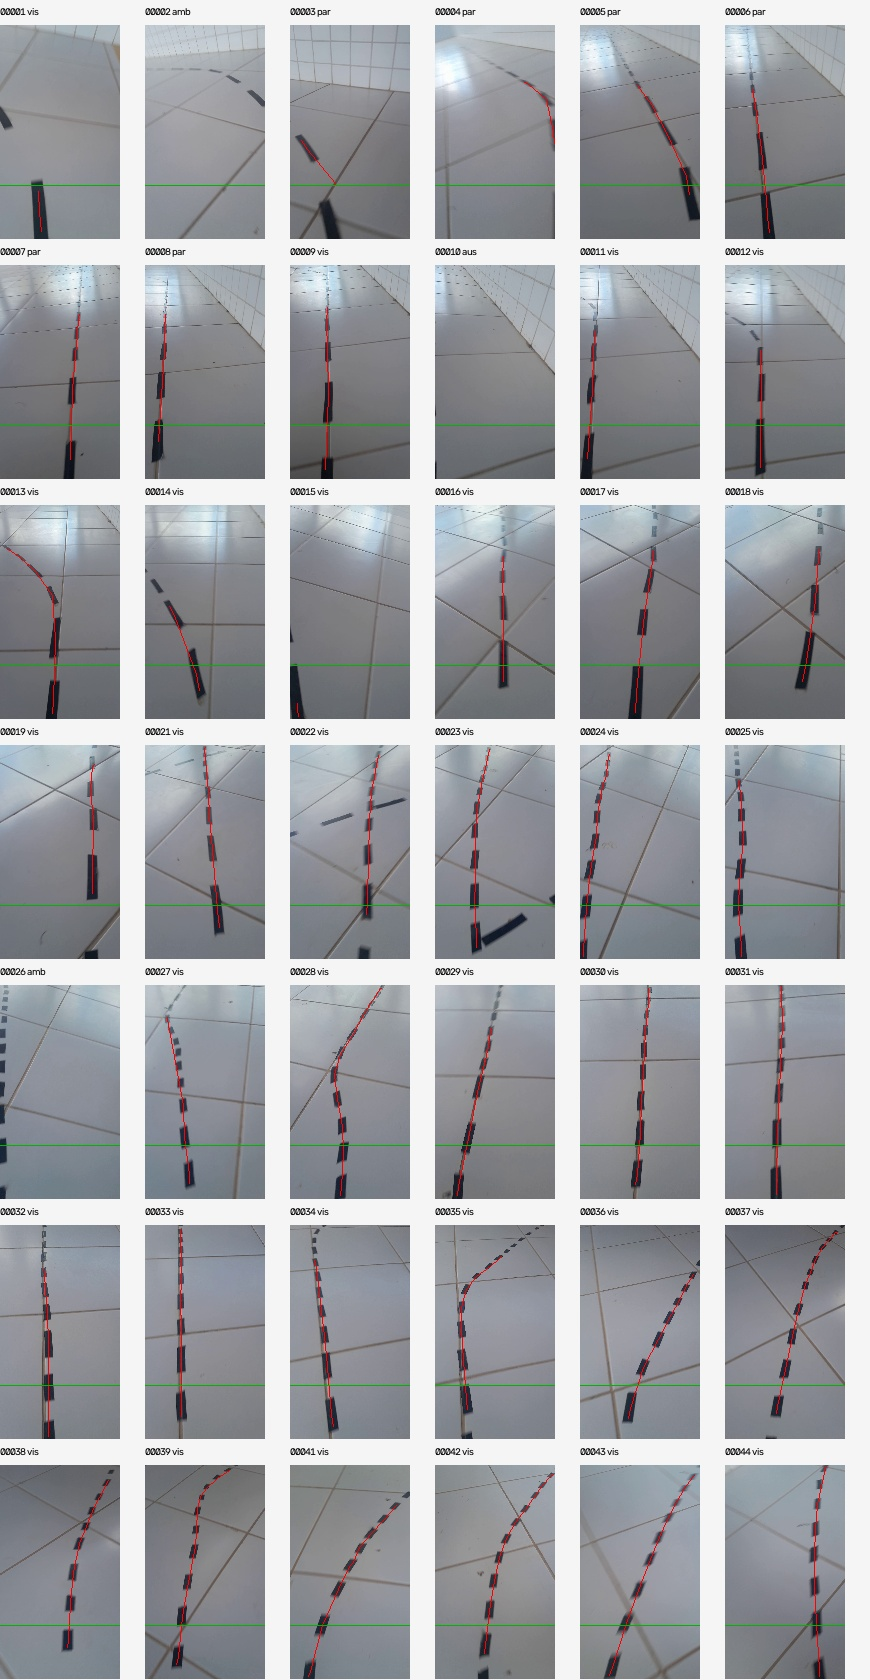
\includegraphics[width=1.0\linewidth,height=0.78\textheight,keepaspectratio]{figuras/novas_marcacoes.jpg}
\caption{Montagem preservada das 42 novas revisões. As marcações humanas definem a referência supervisionada; nem todas as revisões produziram um alvo válido para a regressão.}
\end{figure}

\section{Preparação das entradas e auxílio à rotulagem}
\subsection{Entrada efetiva da CNN}
O recorte utiliza a largura inteira, proporção 2:1 e centro vertical na referência de 75\% da altura. A região é convertida em cinza e redimensionada para 40 linhas por 80 colunas, evitando deformar diretamente toda a imagem vertical. A entrada possui um canal, com tensor $1\times40\times80$ por exemplo.

Após dividir os pixels por 255, aplica-se normalização por imagem:
\begin{equation}
 I_{norm}=\operatorname{clip}\left(\frac{I/255-\mu}{\sigma+0{,}08},-4,4\right).
\end{equation}
A média $\mu$ e o desvio padrão $\sigma$ são calculados na própria imagem. Isso reduz a sensibilidade a brilho e contraste globais, sem eliminar todos os efeitos de iluminação. O alvo é
\begin{equation}
 p=\frac{2x}{W-1}-1,
\end{equation}
com $x$ na imagem original e $W$ sua largura.

\subsection{OpenCV como assistência à marcação}
Foi desenvolvida uma sugestão geométrica da trajetória para revisão humana. A versão revisada reduz proporcionalmente a imagem até 640 pixels no maior lado, estima o fundo por fechamento morfológico elíptico $51\times51$, divide o cinza pelo fundo estimado, suaviza com filtro $3\times3$ e utiliza limiares e abertura para controlar ruído. A seleção dos segmentos considera suporte de pixels, espessura e vãos do tracejado, reduzindo a preferência indevida por vários fragmentos de rejunte.

A sugestão não substitui a confirmação humana. A análise exploratória usou 44 frames de treino e validação, sem os vídeos de teste da CNN. O algoritmo foi ajustado durante o estudo e as revisões assistidas não são cegas ao método.
\begin{table}[ht]\centering\small
\caption{Comparação exploratória da assistência OpenCV. Cobertura e erro devem ser interpretados juntos.}
\begin{tabular}{lrrr}\toprule
Estratégia & Frames com sobreposição & MAE & Cobertura\\\midrule
Anterior &43&0,1187&77,8\%\\
Seleção nova, sem correção &44&0,0142&86,6\%\\
Seleção nova, iluminação corrigida &44&0,0200&92,7\%\\
Seleção nova, CLAHE &44&0,0583&93,6\%\\\bottomrule
\end{tabular}\end{table}
O erro usa até 25 alturas da trajetória humana, somente onde há sobreposição com a sugestão. Na comparação restrita às mesmas alturas em 40 imagens, o MAE foi de 0,0712 no algoritmo anterior e 0,0197 com correção de iluminação. A correção ampliou a cobertura, mas prejudicou algumas imagens. Esses números pertencem à assistência OpenCV, não ao desempenho da CNN. O tratamento de iluminação dessa ferramenta não foi aplicado à entrada da CNN nos experimentos comparados.


\subsection{Registro visual do pré-processamento e da rotulagem}

\begin{figure}[htbp]
\centering
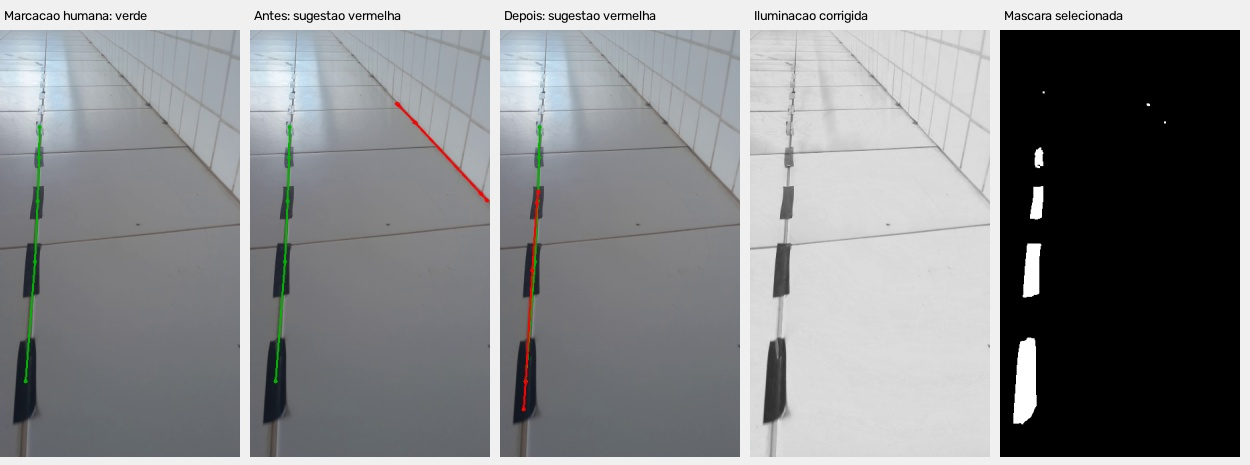
\includegraphics[width=\linewidth]{figuras/diagnostico_video_01_frame_00008.jpg}
\caption{Exemplo de \texttt{preprocessamento\_02/diagnosticos/video\_01\_frame\_00008.jpg}. Da esquerda para a direita: marcação humana em verde; sugestão anterior em vermelho; sugestão revisada em vermelho; imagem com iluminação corrigida; máscara selecionada. A sugestão anterior se desvia para a direita, enquanto a revisada acompanha os segmentos principais da fita no trecho inferior. A máscara evidencia os segmentos separados do tracejado.}
\label{fig:diagnostico-video01-00008}
\end{figure}
A Figura~\ref{fig:diagnostico-video01-00008} documenta uma falha concreta da seleção anterior e a mudança obtida com o tratamento revisado. A aproximação visual da marcação humana nesse frame ilustra o funcionamento da assistência à rotulagem; não constitui uma previsão da CNN nem comprova desempenho em todas as imagens.


A Figura~\ref{fig:diagnostico-pre} mostra um diagnóstico preservado da versão revisada do pré-processamento, para \texttt{video\_07\_frame\_00084.jpg}. Os cinco painéis permitem acompanhar a referência humana, a sugestão anterior, a sugestão nova, o cinza tratado e a máscara. Nesta amostra, o algoritmo anterior seguia o rejunte direito; a seleção revisada acompanha os segmentos principais da trajetória. A comparação é ilustrativa e não garante o mesmo comportamento em todas as imagens.
\begin{figure}[htbp]\centering
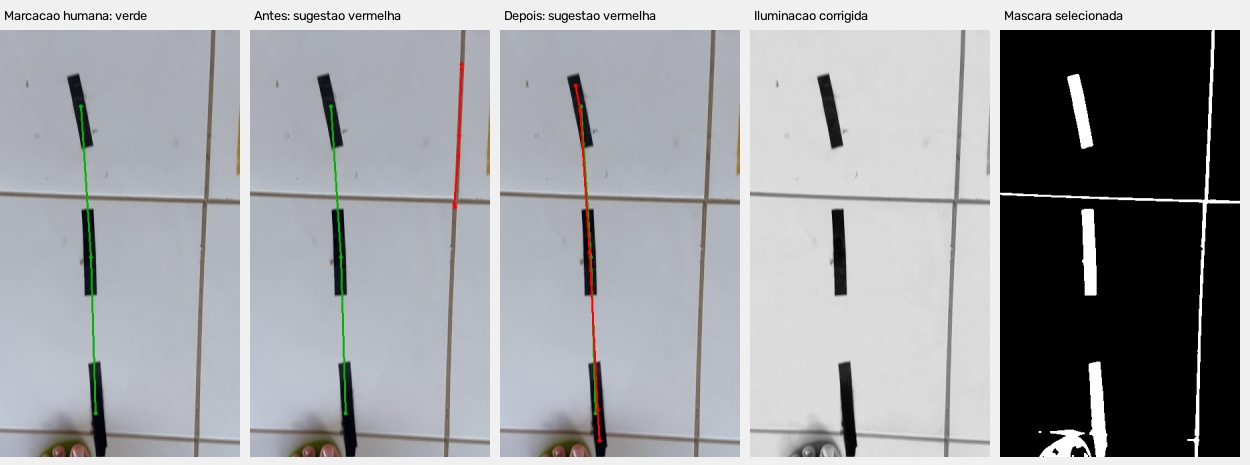
\includegraphics[width=\linewidth]{figuras/diagnostico_preprocessamento.jpg}
\caption{Diagnóstico do pré-processamento extraído da pasta de diagnósticos do segundo estudo. Verde representa a marcação humana; vermelho, a sugestão OpenCV. O cinza tratado e a máscara ajudam a explicar como o contraste e a seleção de segmentos produzem a proposta de trajetória.}
\label{fig:diagnostico-pre}\end{figure}

Na ferramenta \texttt{rotular\_linha.py}, o operador examina a sugestão em ciano, arrasta pontos para corrigir, clica para adicionar pontos e usa o botão direito para removê-los. As edições e revisões salvas aparecem em vermelho. Em seguida, seleciona o estado \texttt{visivel}, \texttt{parcial}, \texttt{ausente} ou \texttt{ambiguo} e utiliza \textit{Confirmar e avançar}. Os controles \textit{Alternar original/tratada}, \textit{Recalcular sugestão} e \textit{Tentar sem correção} auxiliam a inspeção. Salvar uma revisão não inicia treinamento.

A Figura~\ref{fig:rotulagem} apresenta os pontos efetivamente salvos pela ferramenta, sobrepostos à imagem original e à versão tratada. São visualizações produzidas a partir do registro de revisão e da rotina de tratamento atual, não capturas históricas da janela. As coordenadas são preservadas na imagem original; a visualização tratada facilita examinar o contraste sem mudar o sistema de coordenadas da marcação. A trajetória é convertida no alvo da CNN apenas onde os pontos abrangem a altura de referência.
\begin{figure}[p]\centering
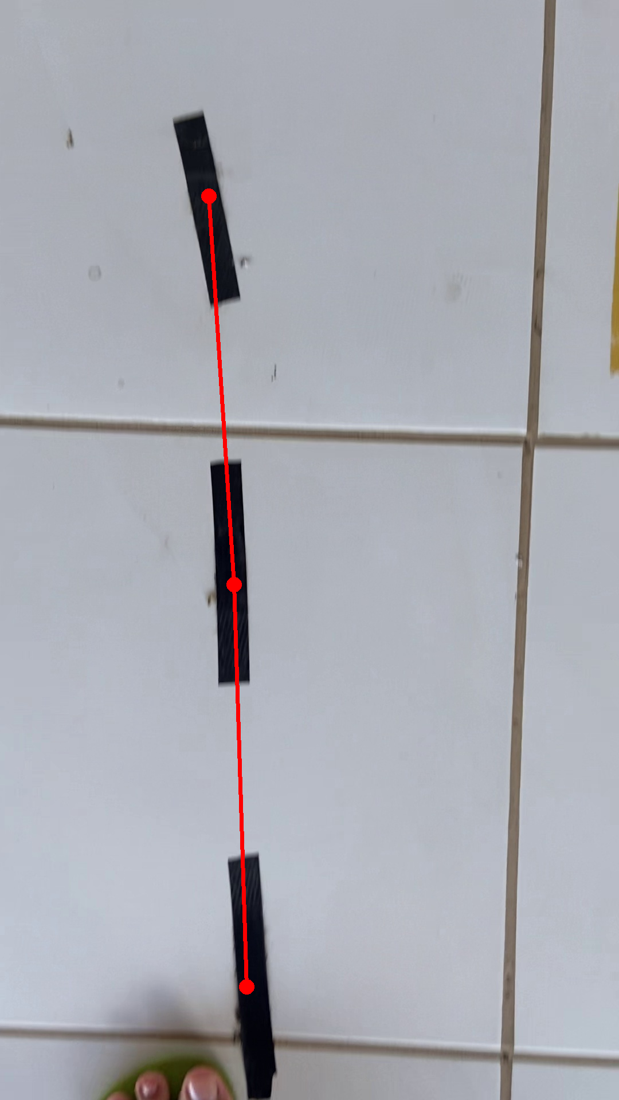
\includegraphics[width=0.47\linewidth,height=0.68\textheight,keepaspectratio]{figuras/rotular_linha_original.png}\hfill
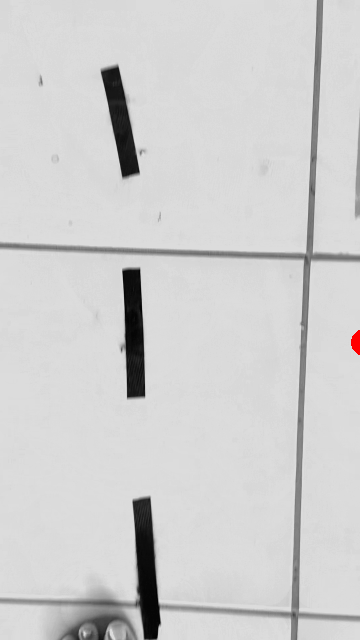
\includegraphics[width=0.47\linewidth,height=0.68\textheight,keepaspectratio]{figuras/rotular_linha_tratada.png}
\caption{Exemplo de revisão salva por \texttt{rotular\_linha.py}: imagem original à esquerda e tratada à direita, ambas com os mesmos pontos humanos em vermelho. Visualização das anotações reais de \texttt{video\_07\_frame\_00084.jpg}, reconstruída para documentar a rotulagem. A interface gráfica não está reproduzida nesta figura.}
\label{fig:rotulagem}\end{figure}

\section{Estrutura da rede neural convolucional}
A rede \texttt{RedeLinha} é implementada em NumPy, com convoluções, retropropagação e otimizador próprios. Os pesos começam aleatórios e não há transferência de aprendizado. A arquitetura possui exatamente 55.090 parâmetros treináveis, incluindo biases.
\begin{table}[ht]\centering
\caption{Arquitetura; dimensões na ordem canais, altura e largura.}
\begin{tabular}{lrrr}\toprule
Camada & Kernel / passo / padding & Saída & Parâmetros\\\midrule
Entrada & -- & $1\times40\times80$ & 0\\
Convolução + ReLU & $5/2/2$ & $8\times20\times40$ & 208\\
Convolução + ReLU & $3/2/1$ & $16\times10\times20$ & 1.168\\
Convolução + ReLU & $3/2/1$ & $16\times5\times10$ & 2.320\\
Flatten & -- & 800 & 0\\
Densa + ReLU & -- & 64 & 51.264\\
Densa & -- & 2 & 130\\\midrule
Total & & & 55.090\\\bottomrule
\end{tabular}\end{table}
As convoluções compartilham filtros entre posições e reduzem progressivamente a resolução usando passo dois. A ReLU aplica $\max(0,z)$; o vetor final de 800 valores alimenta a camada densa. Não há camada de pooling separada, dropout ou normalização de lote nessa implementação.

A primeira saída passa por tangente hiperbólica e fica entre $-1$ e $1$. Embora a implementação geral a denomine direção, neste experimento ela foi supervisionada como posição horizontal. A segunda saída é um logit de visibilidade, convertido por sigmoide na inferência geral. Seu peso de perda foi fixado em zero: a visibilidade não foi treinada nem avaliada e não deve ser interpretada como confiança confiável.


\subsection{Extração de características: técnicas explícitas e aprendizado}
Uma característica, ou \textit{feature}, é uma informação da imagem útil para a tarefa. No problema estudado, diferenças de intensidade, bordas, orientação de segmentos e sua organização espacial podem ajudar a localizar a fita. A imagem contém também características irrelevantes ou enganosas, como rejuntes e sombras. O desafio é construir uma representação que favoreça a trajetória correta.

O fluxo desenvolvido utiliza duas estratégias com papéis diferentes. Na assistência OpenCV, o tratamento e a seleção geométrica são definidos explicitamente no código. Na CNN, os valores dos filtros são ajustados a partir dos exemplos rotulados para reduzir o erro de posição. A CNN dos experimentos recebe o recorte em cinza normalizado; não recebe a máscara, os contornos ou os pontos sugeridos pelo OpenCV como canais adicionais. As marcações humanas fornecem o alvo supervisionado, e não um mapa de características de entrada.

\subsubsection{Características simples no processamento clássico}
A conversão para cinza concentra a análise nas intensidades. A correção de iluminação procura reduzir variações lentas do fundo, enquanto a limiarização produz uma máscara que diferencia regiões escuras do restante da cena. A abertura morfológica ajuda a remover fragmentos finos; a seleção geométrica usa suporte de pixels, espessura e separação entre segmentos para propor uma trajetória. Essas operações explicitam critérios de seleção, em vez de aprendê-los por retropropagação.

A máscara binária é uma representação intermediária, não uma garantia de que seus pixels pertencem à fita. Um rejunte pode satisfazer critérios de intensidade e uma sombra pode formar uma região escura maior que a pista. A combinação de intensidade e geometria procura reduzir essas ambiguidades. O diagnóstico visual incluído neste relatório mostra um caso em que a seleção anterior se afasta da fita, ajudando a justificar a revisão dos critérios.

\subsubsection{Características aprendidas pela convolução}
Na CNN, um filtro percorre regiões locais da entrada e aplica os mesmos pesos em diferentes posições. Para uma camada, a operação pode ser escrita como
\begin{equation}
 Z_{k,i,j}=b_k+\sum_{c=1}^{C_{in}}\sum_{u=0}^{K-1}\sum_{v=0}^{K-1}
 W_{k,c,u,v}\,X_{c,si+u-p,sj+v-p},
\end{equation}
em que $k$ identifica o filtro de saída, $c$ o canal de entrada, $K$ o tamanho do kernel, $s$ o passo e $p$ o preenchimento com zeros. Os valores fora dos limites da entrada são tratados como zero. A implementação realiza essa operação sem inversão espacial do kernel, conforme a convenção usual de camadas convolucionais em redes neurais.

Cada filtro produz um mapa de ativação. Um valor elevado indica resposta forte ao padrão representado pelos pesos naquela região; não é, por si só, uma probabilidade de presença da linha. O compartilhamento de pesos permite procurar o mesmo padrão em diversas posições sem aprender um conjunto independente de coeficientes para cada pixel.

Depois de cada convolução, a ReLU aplica $A=\max(0,Z)$. Essa não linearidade permite que a composição das camadas represente relações que uma sequência de transformações puramente lineares não representaria. Os filtros começam aleatórios: bordas ou segmentos não são fornecidos como detectores prontos. Eles podem surgir como padrões úteis ao reduzir a perda supervisionada.

\subsection{Hierarquia de características na arquitetura utilizada}
\subsubsection{Primeira convolução: padrões locais simples}
A primeira camada possui oito filtros $5\times5$, um canal de entrada e passo dois. Sua saída contém oito mapas de $20\times40$. Cada ativação depende de uma vizinhança pequena da imagem de $40\times80$ pixels. Nessa etapa, respostas a transições entre claro e escuro, bordas orientadas, manchas e texturas locais são exemplos de características que podem ser úteis.

No caso da fita escura sobre piso claro, suas bordas geram contrastes locais. Porém, os rejuntes também podem gerar contrastes semelhantes. A primeira camada não deve ser interpretada como uma solução completa de reconhecimento da pista: seus padrões locais precisam ser combinados com informações de outras regiões e camadas.

\subsubsection{Segunda convolução: combinação de padrões}
A segunda camada possui 16 filtros $3\times3$, cada um combinando os oito canais anteriores, e produz 16 mapas de $10\times20$. Portanto, seus filtros não atuam diretamente nos pixels originais; atuam nas respostas aprendidas pela primeira camada. Essa combinação permite representar relações entre bordas, contraste e orientação em uma região maior.

Para a tarefa estudada, candidatos a características intermediárias incluem pares de bordas delimitando uma faixa e configurações locais compatíveis com segmentos da fita. São exemplos interpretativos de padrões possíveis, não descrições verificadas dos filtros treinados. Uma rede com poucos dados também pode aprender relações espúrias com o piso ou a iluminação.

\subsubsection{Terceira convolução: estruturas de maior contexto}
A terceira camada combina os 16 canais anteriores com 16 filtros $3\times3$ e gera mapas de $5\times10$. Suas ativações podem integrar informações locais mais abrangentes, relacionadas à organização de segmentos, continuidade aparente e posição de estruturas no recorte. O termo característica complexa indica aqui uma composição de padrões anteriores, e não uma garantia de compreensão semântica da pista.

Uma única ativação dessa camada ainda não observa todo o recorte. Além disso, a saída final da rede é somente uma coordenada horizontal: os experimentos não supervisionaram segmentação pixel a pixel, identificação de cruzamentos ou classificação de tipos de curva. Não se pode atribuir essas capacidades ao modelo apenas por ele possuir três convoluções.

\subsubsection{Campo receptivo e aumento de contexto}
O campo receptivo teórico é a região da entrada que pode influenciar uma ativação. Para kernels $k_l$ e passos $s_l$, usando $r_0=j_0=1$, seu tamanho e o espaçamento entre centros são
\begin{equation}
 r_l=r_{l-1}+(k_l-1)j_{l-1},\qquad
 j_l=j_{l-1}s_l.
\end{equation}
Aplicando a fórmula às três convoluções implementadas, obtêm-se os valores da Tabela~\ref{tab:campo-receptivo}. Eles são expressos em pixels da entrada reduzida, não da fotografia original. Nas bordas, parte do suporte corresponde ao preenchimento com zeros. O campo receptivo teórico descreve dependências possíveis e não mede quais pixels efetivamente dominaram a decisão.
\begin{table}[htbp]\centering
\caption{Progressão do contexto espacial nas convoluções da CNN utilizada.}
\label{tab:campo-receptivo}
\begin{tabular}{lccc}\toprule
Etapa & Mapas de saída & Campo receptivo & Espaçamento\\\midrule
Convolução 1 & $8\times20\times40$ & $5\times5$ & 2 pixels\\
Convolução 2 & $16\times10\times20$ & $9\times9$ & 4 pixels\\
Convolução 3 & $16\times5\times10$ & $17\times17$ & 8 pixels\\\bottomrule
\end{tabular}
\end{table}

\subsubsection{Camadas densas: integração e regressão da posição}
O \textit{flatten} reorganiza os 16 mapas de $5\times10$ em 800 valores sem aprender parâmetros. A camada densa de 64 unidades combina esses valores de todas as posições. Assim, a decisão final pode integrar informações distribuídas por todo o recorte, mesmo que cada ativação convolucional tenha suporte local.

Essa etapa preserva a possibilidade de distinguir posições espaciais: a localização horizontal importa para a regressão. A camada final produz dois valores; a tangente hiperbólica da primeira saída gera a posição normalizada. O gradiente da perda compara essa posição com o alvo humano e atualiza tanto as camadas densas quanto os filtros convolucionais. As características são aprendidas em função da tarefa de localização, sem rótulos individuais de borda, textura ou segmento.

A maior parte dos parâmetros está na primeira camada densa: 51.264 de 55.090, aproximadamente 93,1\%. Isso ajuda a entender por que mesmo esta CNN pequena pode ajustar particularidades de um conjunto com poucas dezenas de imagens. A hierarquia convolucional não elimina o risco de sobreajuste.

\subsection{O que os resultados demonstram sobre as características}
A redução do MAE no conjunto exploratório é compatível com o aprendizado de uma representação útil para localizar a linha nesses frames. Entretanto, ela não revela diretamente quais filtros detectam bordas nem quais ativações respondem à fita. As imagens de previsão apresentadas neste relatório mostram a coordenada estimada; os diagnósticos do OpenCV mostram o processamento clássico. Nenhuma dessas imagens é um mapa interno de ativação da CNN.

Neste trabalho não foi realizada inspeção dos filtros ou dos mapas intermediários. Portanto, a associação entre primeiras camadas e características simples, e entre camadas posteriores e combinações mais complexas, explica a estrutura e suas possibilidades; não constitui uma observação experimental específica dos pesos obtidos.

Uma extensão útil seria visualizar os oito filtros da primeira camada e os mapas de ativação das três convoluções para o mesmo frame. Comparar frames com fita, rejunte, sombra e ausência de linha permitiria investigar a que regiões cada canal responde. Outra análise possível seria ocultar pequenas regiões da entrada e medir a variação da coordenada estimada, verificando a sensibilidade da previsão. Essas análises devem acompanhar os erros de posição e não substituir a validação com gravações independentes e câmera real.

\section{Protocolo de treinamento}
Os dois experimentos partiram do zero com a mesma semente sete, lote de oito exemplos, taxa de aprendizado 0,001 e orçamento de 300 atualizações. Foi utilizado Adam, com $\beta_1=0,9$, $\beta_2=0,999$, $\epsilon=10^{-8}$ e regularização L2 de $10^{-4}$ nos pesos. O aumento de dados usa espelhamento horizontal com probabilidade de 50\%, invertendo o sinal do alvo, e ruído gaussiano de desvio padrão 0,05 na entrada normalizada.

A perda de posição é Huber, com $\delta=0,3$:
\begin{equation}
 L_\delta(e)=\begin{cases}\frac12e^2,&|e|\leq\delta,\\
 \delta(|e|-\frac12\delta),&|e|>\delta.
 \end{cases}
\end{equation}
O termo de visibilidade foi desativado. A validação é calculada a cada dez atualizações. O checkpoint é escolhido pelo menor MSE de validação, resultando no passo 170 no primeiro treino e 130 no segundo. O teste é avaliado após a seleção em cada execução. Entretanto, as imagens de teste já haviam sido vistas na exploração do projeto; esse protocolo não transforma o conjunto em teste final intocado.

Manter 300 atualizações não iguala o número de épocas quando o dataset aumenta. A comparação representa um orçamento igual de atualizações, com maior diversidade de exemplos no segundo treino. Não permite isolar causalmente o efeito da quantidade de dados, pois a distribuição de posições e a forma de rotular também mudaram.

\section{Resultados quantitativos}
\subsection{Definição das métricas}
Para $N$ exemplos, $\mathrm{MAE}=N^{-1}\sum_i|\hat p_i-p_i|$ e $\mathrm{MSE}=N^{-1}\sum_i(\hat p_i-p_i)^2$. Como a coordenada normalizada cobre uma largura de aproximadamente duas unidades, o erro percentual da largura é $50\,\mathrm{MAE}$. Mais precisamente, a conversão para pixels da imagem original é $|\hat p-p|(W-1)/2$. Assim, MAE de 0,1 equivale aproximadamente a 5\% da largura.

Não há classificação de categorias nesta tarefa. Portanto, MAE de 3,6\% da largura não significa acurácia de 96,4\%, e matriz de confusão não é a medida apropriada para essa regressão.
\begin{table}[ht]\centering\caption{Resultados dos checkpoints selecionados.}\begin{tabular}{llrrrr}\toprule Experimento & Conjunto & N & MAE & MSE & MAE (\% largura)\\\midrule
1 & treino & 24 & 0.0201 & 0.0006 & 1.01\\
1 & validacao & 10 & 0.1403 & 0.0303 & 7.02\\
1 & teste & 9 & 0.1373 & 0.0489 & 6.87\\
2 & treino & 58 & 0.0349 & 0.0020 & 1.75\\
2 & validacao & 10 & 0.1026 & 0.0146 & 5.13\\
2 & teste & 9 & 0.0725 & 0.0096 & 3.62\\
\bottomrule\end{tabular}\end{table}
\subsection{Comparação e referências simples}
O MAE de teste diminuiu de 0,1373 para 0,0725, redução relativa de aproximadamente 47,2\%. O MSE passou de 0,0489 para 0,0096. O pior erro absoluto normalizado caiu de 0,5963 para 0,2462, ainda equivalente a aproximadamente 12,3\% da largura no segundo experimento. Quatro das nove imagens de teste melhoraram; o ganho agregado não representa melhora uniforme.

No segundo experimento, prever sempre o centro produz MAE 0,2322 no teste; prever sempre a média dos alvos de treino produz 0,2358. A CNN, com 0,0725, supera essas referências nesse pequeno conjunto. Isso mostra informação útil nas previsões observadas, mas não estabelece robustez em outras pistas ou dispositivos.

O erro de treino menor que o de validação indica uma diferença entre ajuste e desempenho fora do treino. O aumento do MAE de treino entre os experimentos não é, sozinho, regressão do método: o conjunto de treino mudou e passou a incluir mais posições. A escolha do checkpoint depende da validação, não do menor erro no treino.

\begin{figure}[p]\centering
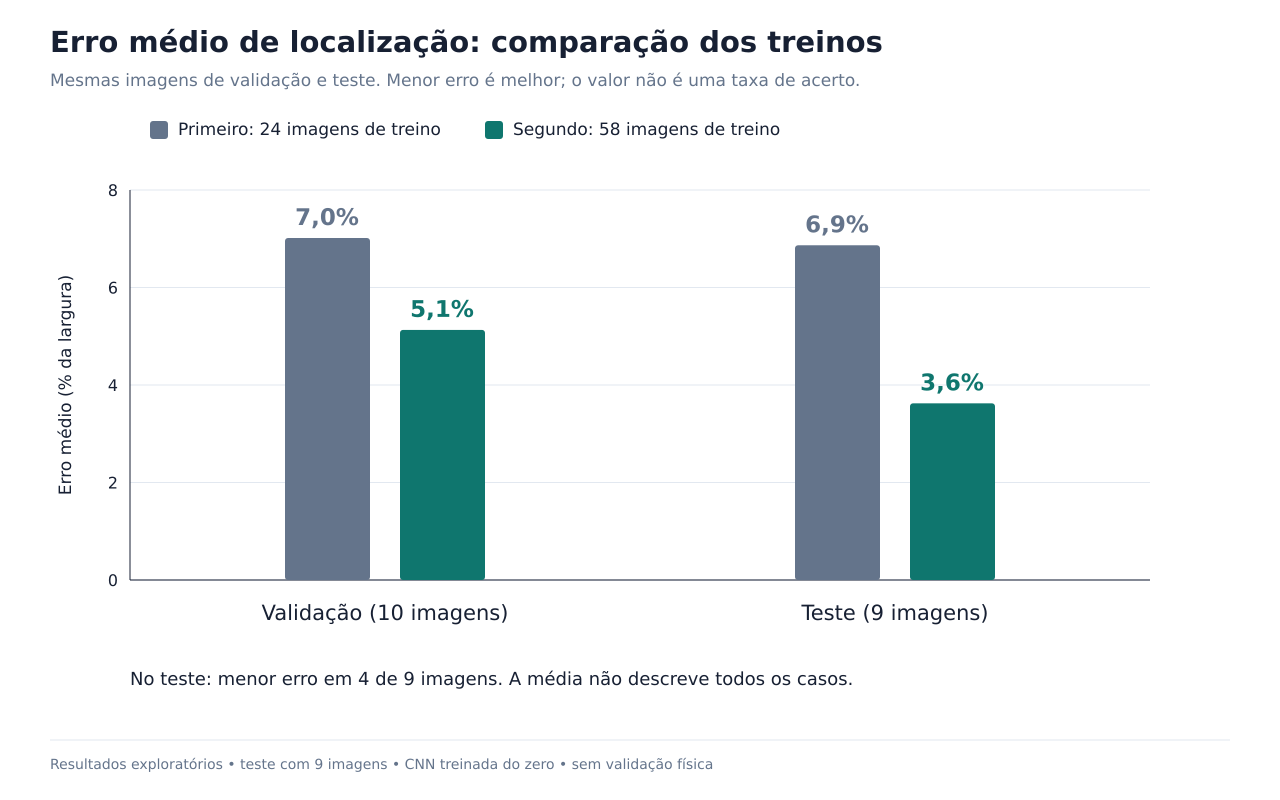
\includegraphics[width=1.0\linewidth,height=0.78\textheight,keepaspectratio]{figuras/01_resumo.png}
\caption{Síntese da comparação dos dois treinos. As barras de erro representam distância média como fração da largura, não taxa de classificação correta.}
\end{figure}

\begin{figure}[p]\centering
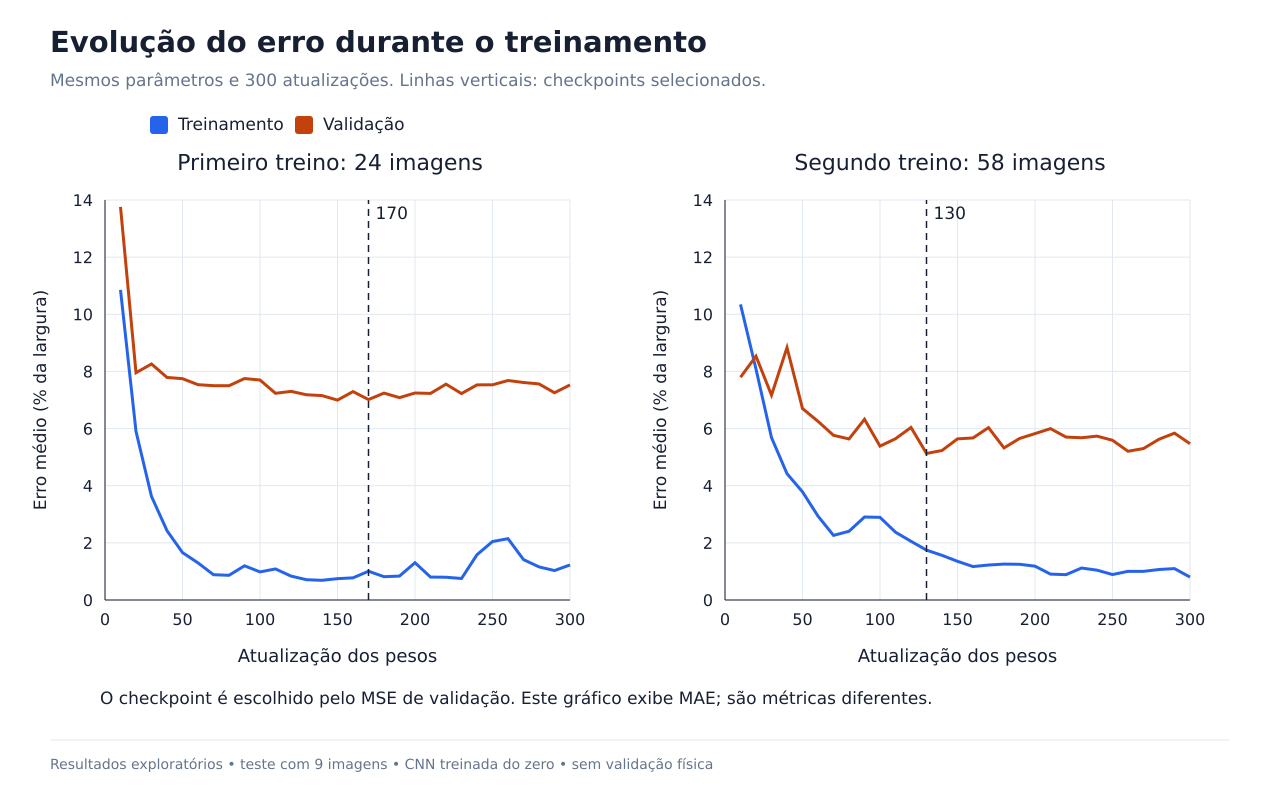
\includegraphics[width=1.0\linewidth,height=0.78\textheight,keepaspectratio]{figuras/02_curvas_treinamento.png}
\caption{Curvas registradas durante as 300 atualizações. A seleção é feita pelo MSE de validação; os checkpoints dos experimentos são distintos.}
\end{figure}

\begin{figure}[p]\centering
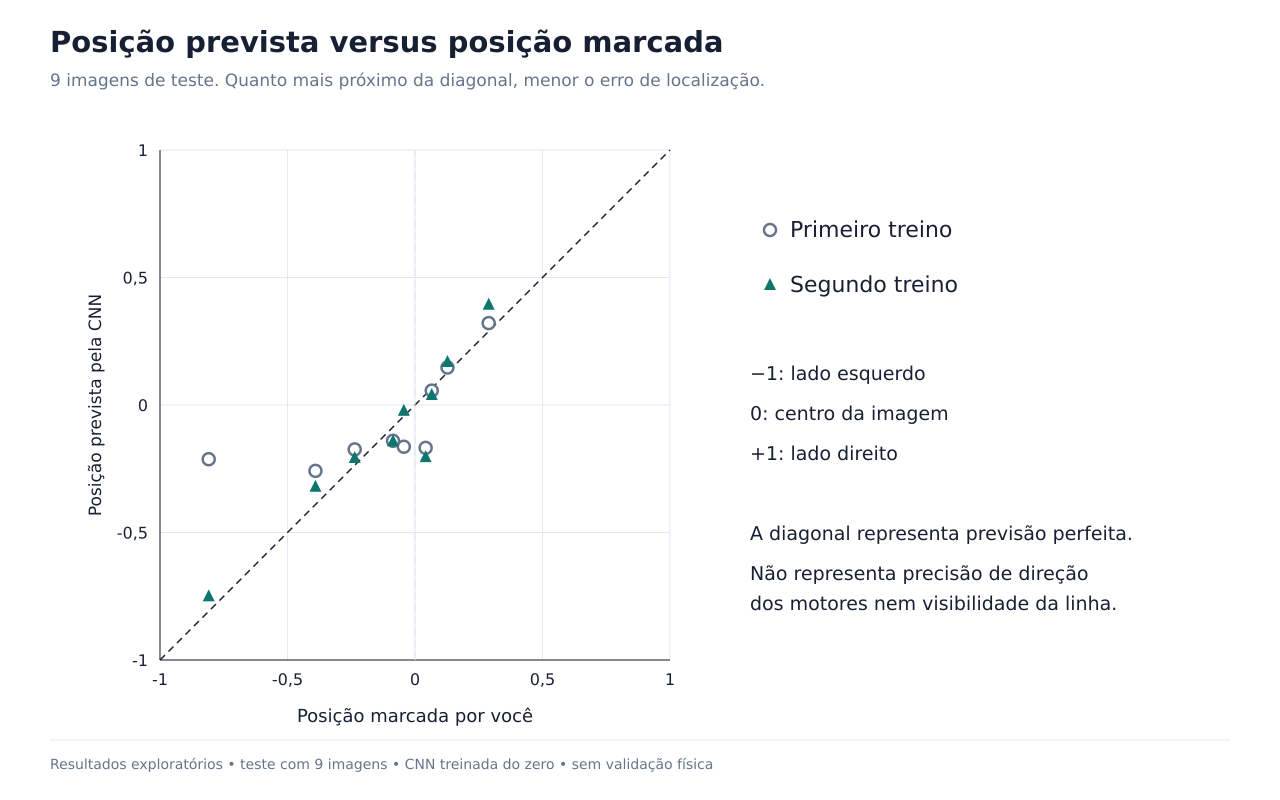
\includegraphics[width=1.0\linewidth,height=0.78\textheight,keepaspectratio]{figuras/03_previsto_real.png}
\caption{Comparação entre posição estimada e referência humana. Distância da diagonal indica erro de localização.}
\end{figure}

\begin{figure}[p]\centering
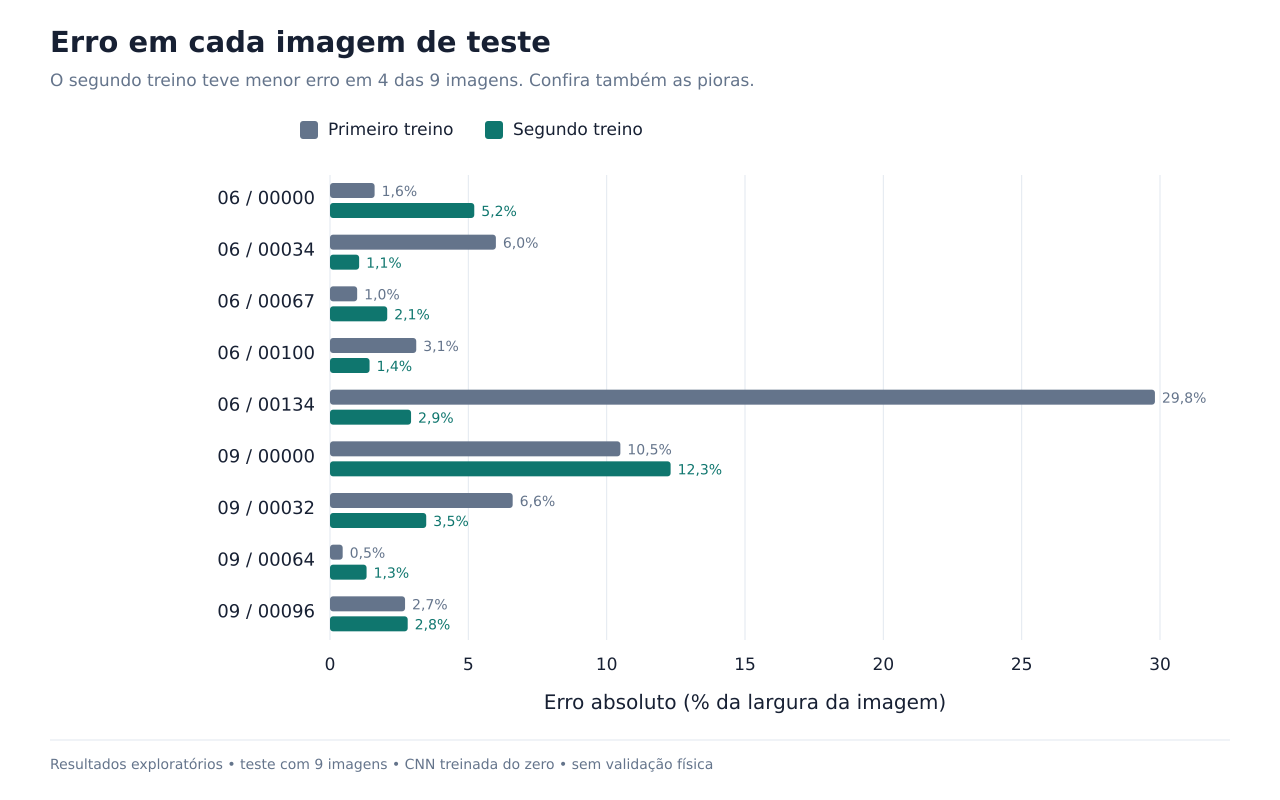
\includegraphics[width=1.0\linewidth,height=0.78\textheight,keepaspectratio]{figuras/04_erros_por_imagem.png}
\caption{Erros nas mesmas imagens de avaliação. A melhora média deve ser confrontada com os casos individuais que pioraram.}
\end{figure}

\begin{figure}[p]\centering
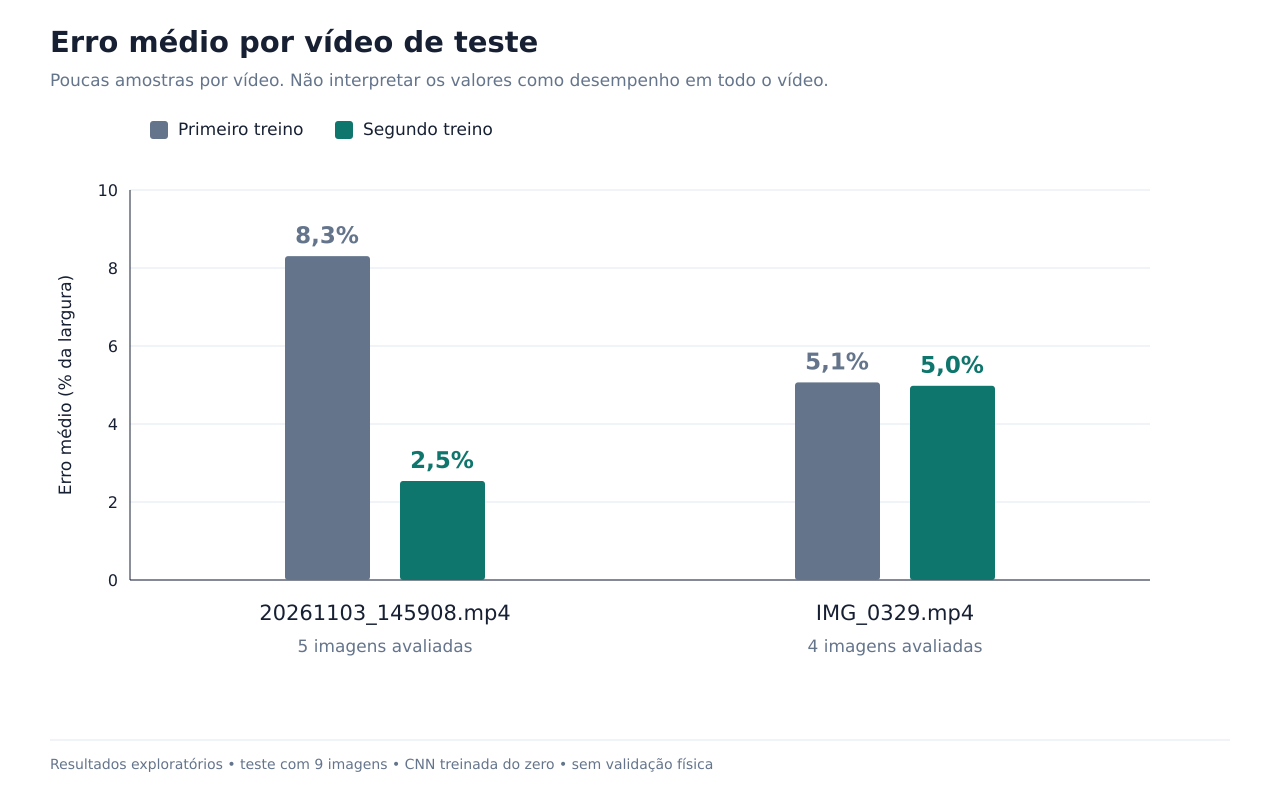
\includegraphics[width=1.0\linewidth,height=0.78\textheight,keepaspectratio]{figuras/05_erros_por_video.png}
\caption{Erro agregado por vídeo de avaliação. Cada média se apoia em poucos frames e não estima desempenho populacional.}
\end{figure}

\begin{figure}[p]\centering
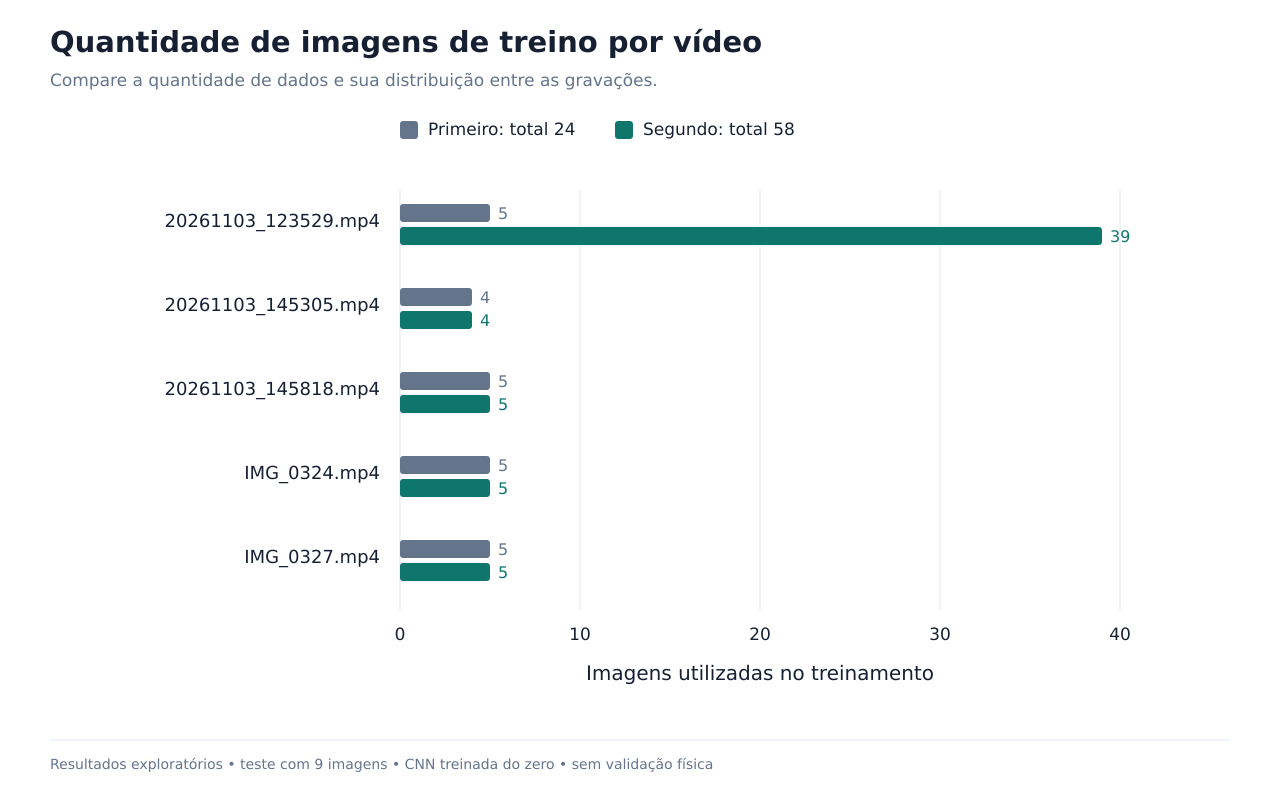
\includegraphics[width=1.0\linewidth,height=0.78\textheight,keepaspectratio]{figuras/06_dados_por_video.png}
\caption{Distribuição das imagens utilizadas por vídeo. A ampliação do treino ficou concentrada no primeiro vídeo.}
\end{figure}
\clearpage\section{Análise detalhada dos nove frames de teste}
A tabela e os pares de imagens a seguir incluem todos os frames de teste. Cada par apresenta o primeiro experimento à esquerda e o segundo à direita. Verde indica marcação humana, a cruz vermelha indica a CNN, azul indica o centro e amarelo delimita o recorte. As sobreposições são as previsões preservadas de cada execução.
\begin{longtable}{lrrr}\toprule Frame & Real & Previsto 2 & Erro 1 / 2 (\% largura)\\\midrule
video\_06\_frame\_00000 & 0.289 & 0.393 & 1.61 / 5.21\\
video\_06\_frame\_00034 & -0.044 & -0.023 & 6.00 / 1.05\\
video\_06\_frame\_00067 & 0.127 & 0.169 & 0.98 / 2.07\\
video\_06\_frame\_00100 & -0.237 & -0.208 & 3.12 / 1.43\\
video\_06\_frame\_00134 & -0.809 & -0.750 & 29.82 / 2.93\\
video\_09\_frame\_00000 & 0.042 & -0.204 & 10.50 / 12.31\\
video\_09\_frame\_00032 & -0.390 & -0.321 & 6.60 / 3.48\\
video\_09\_frame\_00064 & 0.066 & 0.039 & 0.46 / 1.32\\
video\_09\_frame\_00096 & -0.086 & -0.142 & 2.71 / 2.81\\
\bottomrule\end{longtable}
\begin{figure}[p]\centering
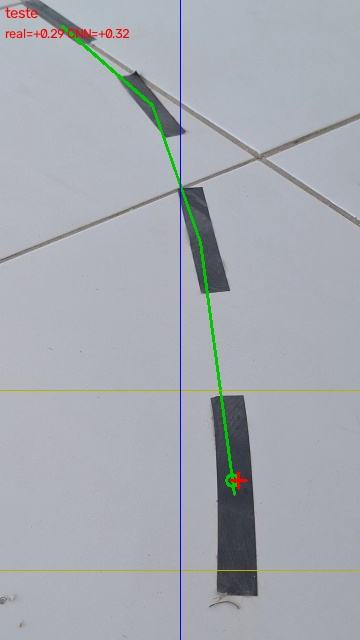
\includegraphics[width=0.47\linewidth,height=0.65\textheight,keepaspectratio]{figuras/exp1_video_06_frame_00000.jpg}
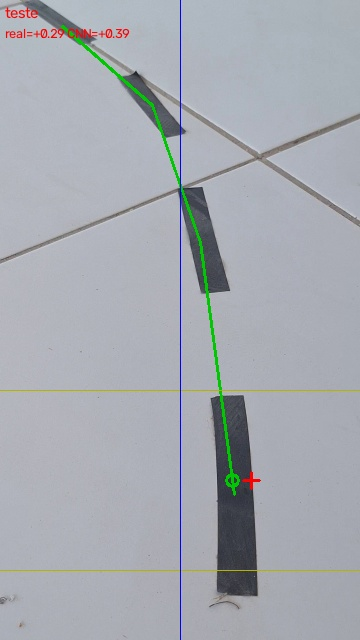
\includegraphics[width=0.47\linewidth,height=0.65\textheight,keepaspectratio]{figuras/exp2_video_06_frame_00000.jpg}
\caption{video\_06\_frame\_00000.jpg: experimento 1 à esquerda e 2 à direita. Erro de 1.61\% para 5.21\% da largura; piora nesta amostra. A referência humana normalizada é 0.289, e a previsão do segundo treino é 0.393.}\end{figure}

\begin{figure}[p]\centering
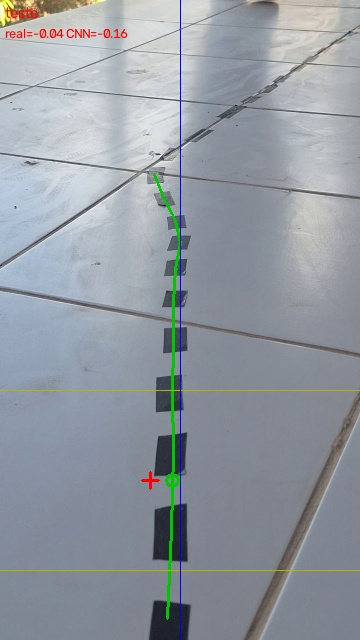
\includegraphics[width=0.47\linewidth,height=0.65\textheight,keepaspectratio]{figuras/exp1_video_06_frame_00034.jpg}
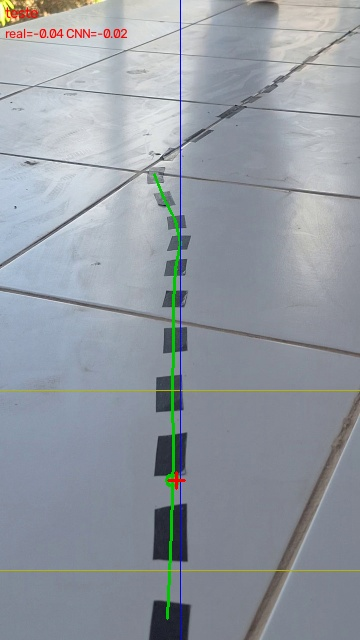
\includegraphics[width=0.47\linewidth,height=0.65\textheight,keepaspectratio]{figuras/exp2_video_06_frame_00034.jpg}
\caption{video\_06\_frame\_00034.jpg: experimento 1 à esquerda e 2 à direita. Erro de 6.00\% para 1.05\% da largura; melhora nesta amostra. A referência humana normalizada é -0.044, e a previsão do segundo treino é -0.023.}\end{figure}

\begin{figure}[p]\centering
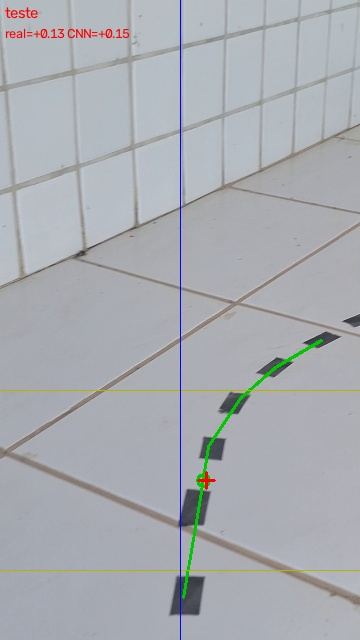
\includegraphics[width=0.47\linewidth,height=0.65\textheight,keepaspectratio]{figuras/exp1_video_06_frame_00067.jpg}
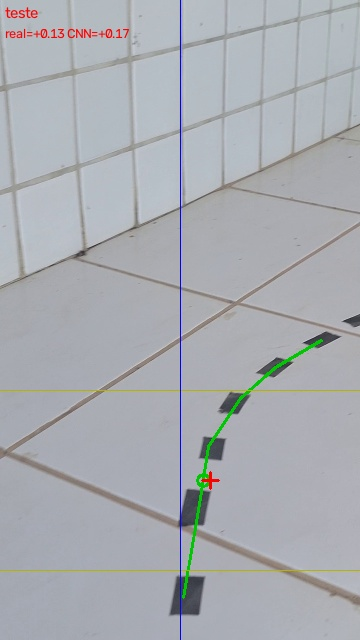
\includegraphics[width=0.47\linewidth,height=0.65\textheight,keepaspectratio]{figuras/exp2_video_06_frame_00067.jpg}
\caption{video\_06\_frame\_00067.jpg: experimento 1 à esquerda e 2 à direita. Erro de 0.98\% para 2.07\% da largura; piora nesta amostra. A referência humana normalizada é 0.127, e a previsão do segundo treino é 0.169.}\end{figure}

\begin{figure}[p]\centering
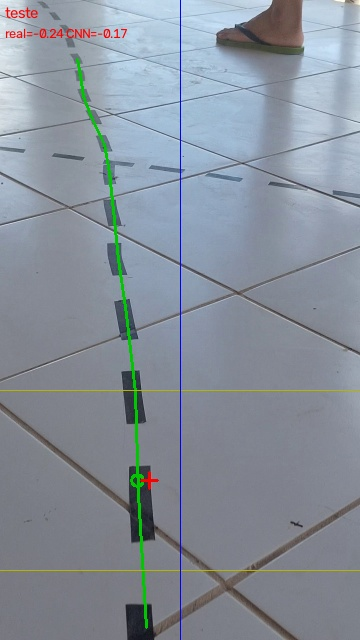
\includegraphics[width=0.47\linewidth,height=0.65\textheight,keepaspectratio]{figuras/exp1_video_06_frame_00100.jpg}
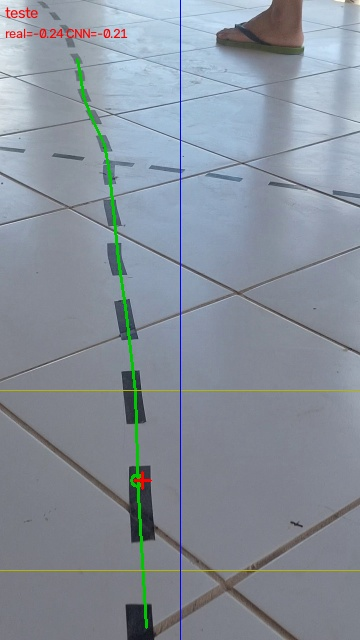
\includegraphics[width=0.47\linewidth,height=0.65\textheight,keepaspectratio]{figuras/exp2_video_06_frame_00100.jpg}
\caption{video\_06\_frame\_00100.jpg: experimento 1 à esquerda e 2 à direita. Erro de 3.12\% para 1.43\% da largura; melhora nesta amostra. A referência humana normalizada é -0.237, e a previsão do segundo treino é -0.208.}\end{figure}

\begin{figure}[p]\centering
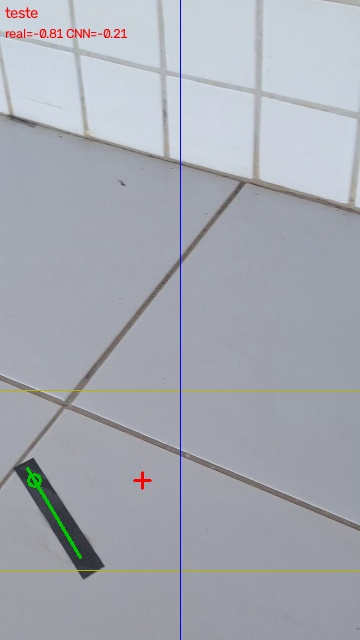
\includegraphics[width=0.47\linewidth,height=0.65\textheight,keepaspectratio]{figuras/exp1_video_06_frame_00134.jpg}
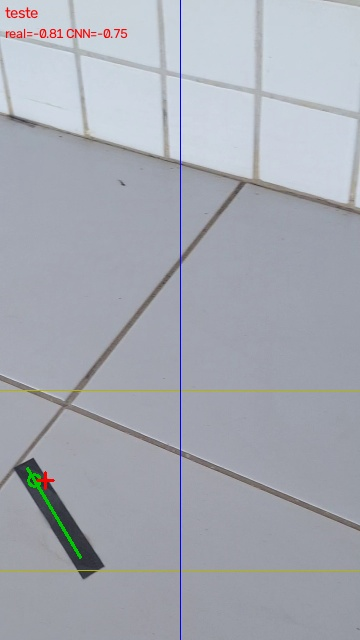
\includegraphics[width=0.47\linewidth,height=0.65\textheight,keepaspectratio]{figuras/exp2_video_06_frame_00134.jpg}
\caption{video\_06\_frame\_00134.jpg: experimento 1 à esquerda e 2 à direita. Erro de 29.82\% para 2.93\% da largura; melhora nesta amostra. A referência humana normalizada é -0.809, e a previsão do segundo treino é -0.750.}\end{figure}

\begin{figure}[p]\centering
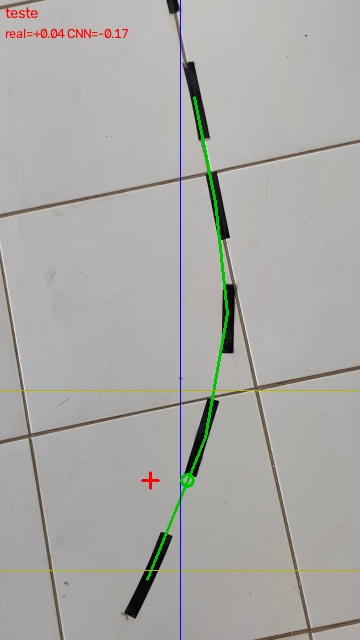
\includegraphics[width=0.47\linewidth,height=0.65\textheight,keepaspectratio]{figuras/exp1_video_09_frame_00000.jpg}
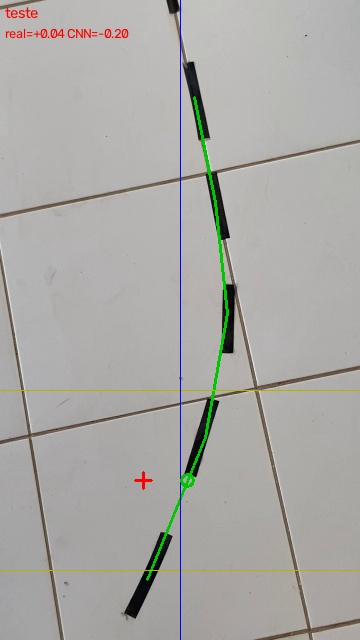
\includegraphics[width=0.47\linewidth,height=0.65\textheight,keepaspectratio]{figuras/exp2_video_09_frame_00000.jpg}
\caption{video\_09\_frame\_00000.jpg: experimento 1 à esquerda e 2 à direita. Erro de 10.50\% para 12.31\% da largura; piora nesta amostra. A referência humana normalizada é 0.042, e a previsão do segundo treino é -0.204.}\end{figure}

\begin{figure}[p]\centering
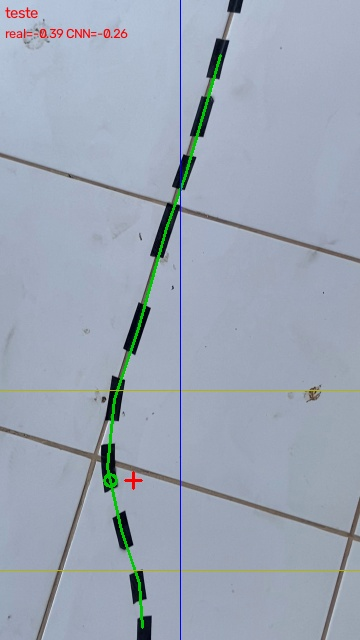
\includegraphics[width=0.47\linewidth,height=0.65\textheight,keepaspectratio]{figuras/exp1_video_09_frame_00032.jpg}
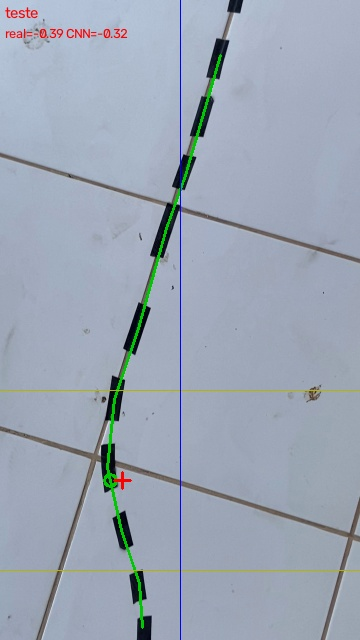
\includegraphics[width=0.47\linewidth,height=0.65\textheight,keepaspectratio]{figuras/exp2_video_09_frame_00032.jpg}
\caption{video\_09\_frame\_00032.jpg: experimento 1 à esquerda e 2 à direita. Erro de 6.60\% para 3.48\% da largura; melhora nesta amostra. A referência humana normalizada é -0.390, e a previsão do segundo treino é -0.321.}\end{figure}

\begin{figure}[p]\centering
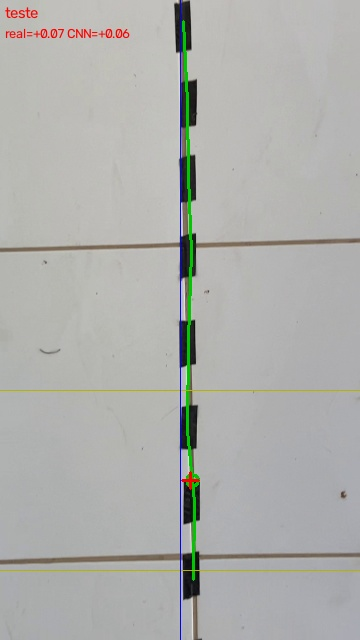
\includegraphics[width=0.47\linewidth,height=0.65\textheight,keepaspectratio]{figuras/exp1_video_09_frame_00064.jpg}
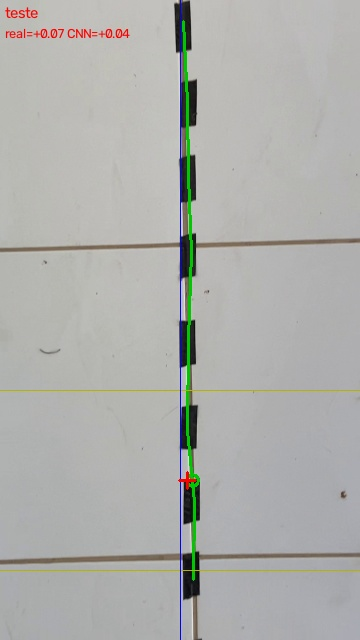
\includegraphics[width=0.47\linewidth,height=0.65\textheight,keepaspectratio]{figuras/exp2_video_09_frame_00064.jpg}
\caption{video\_09\_frame\_00064.jpg: experimento 1 à esquerda e 2 à direita. Erro de 0.46\% para 1.32\% da largura; piora nesta amostra. A referência humana normalizada é 0.066, e a previsão do segundo treino é 0.039.}\end{figure}

\begin{figure}[p]\centering
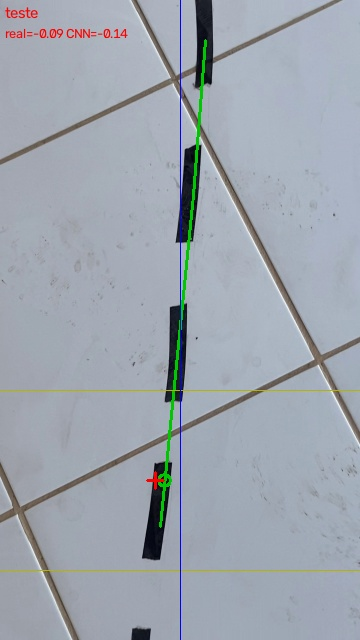
\includegraphics[width=0.47\linewidth,height=0.65\textheight,keepaspectratio]{figuras/exp1_video_09_frame_00096.jpg}
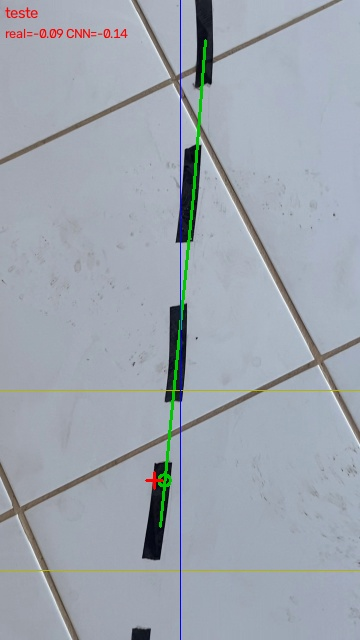
\includegraphics[width=0.47\linewidth,height=0.65\textheight,keepaspectratio]{figuras/exp2_video_09_frame_00096.jpg}
\caption{video\_09\_frame\_00096.jpg: experimento 1 à esquerda e 2 à direita. Erro de 2.71\% para 2.81\% da largura; piora nesta amostra. A referência humana normalizada é -0.086, e a previsão do segundo treino é -0.142.}\end{figure}

\clearpage
\section{Limitações e melhorias propostas}
\subsection{Diversidade e independência dos dados}
A prioridade é coletar gravações independentes com a câmera que será usada no robô, mantendo altura, inclinação, lente e resolução de operação. Devem ser incluídas curvas, cruzamentos, fita interrompida, sombras, reflexos, diferentes pisos, velocidades e situações sem linha. Novos frames consecutivos de uma única gravação aumentam a contagem, mas acrescentam menos diversidade do que novas sessões de captura.

Recomenda-se equilibrar posições à esquerda, ao centro e à direita, limitar a concentração por vídeo e revisar especialmente os maiores erros. Os critérios de anotação em cruzamentos devem definir qual trajetória seguir. Uma segunda revisão de parte dos rótulos ajudaria a medir ambiguidade e inconsistência humana.

Uma próxima avaliação deve reservar vídeos nunca usados na escolha de pré-processamento, rótulos ou parâmetros. O teste atual pode continuar como conjunto exploratório de regressão, mas não como evidência final independente. Com mais gravações, validação cruzada agrupada por vídeo e múltiplas sementes podem avaliar estabilidade; intervalos de incerteza devem considerar a correlação entre frames.

\subsection{Modelo e métricas}
Antes de ampliar a arquitetura, convém aumentar a diversidade e analisar os erros. Podem ser investigados aumentos de brilho, contraste, desfoque e perspectiva que preservem a geometria do alvo. Alterações no recorte devem ser comparadas sob um protocolo fixo, pois podem remover contexto importante em curvas e cruzamentos.

A saída de visibilidade exige exemplos de presença e ausência, supervisão explícita e avaliação própria. Sem isso, não há base para usá-la como mecanismo de confiança. Para a posição, além de MAE e MSE, é útil acompanhar mediana, percentis altos e proporção de frames abaixo de tolerâncias geométricas definidas previamente. Esses indicadores ainda precisam ser calculados em um conjunto representativo.

\subsection{Da avaliação offline à câmera e ao controle}
Os testes apresentados foram realizados em frames já gravados. Não medem latência ponta a ponta, taxa de captura, perdas de comunicação, vibração da câmera ou comportamento dos motores. Também não medem a capacidade de completar voltas na pista.

A transição pode começar pela câmera real com o robô parado, registrando imagens e previsões sem acionar motores. Depois, deve-se verificar a correspondência entre o recorte de treinamento e o fluxo da câmera, medir tempo de processamento e reavaliar o modelo com novas marcações. A função geral de entrada da câmera e o recorte usado neste experimento possuem caminhos diferentes; essa compatibilidade precisa ser conferida antes da integração.

Somente após validar a percepção deve-se definir a conversão de posição em comando, calibrar ganhos e testar em baixa velocidade com parada supervisionada. O desempenho físico deve incluir desvio lateral, perdas da linha, intervenções e conclusão de percursos. Suavização temporal pode reduzir oscilação, mas precisa ser avaliada quanto ao atraso nas curvas. Estas são propostas futuras, não resultados já obtidos.

\section{Conclusão}
Foi construído um fluxo rastreável de preparação de frames, revisão humana, treinamento e avaliação offline de uma CNN pequena. Com arquitetura constante, o segundo experimento apresentou menor erro médio no conjunto exploratório de teste, passando de aproximadamente 6,9\% para 3,6\% da largura. A inspeção individual mostra melhora em quatro frames e piora em cinco, reforçando a necessidade de analisar distribuições e casos difíceis.

A principal entrega é uma evidência inicial de localização horizontal supervisionada, acompanhada de dados e previsões verificáveis. A amostra pequena, a concentração em um vídeo e a consulta prévia ao teste impedem concluir generalização. A etapa com câmera real, supervisão da visibilidade e validação do controle físico permanece pendente. Os pesos experimentais não foram ativados no carrinho.

\appendix
\section{Fontes locais e reprodução}
Os resultados provêm dos arquivos \texttt{experimento.json}, \texttt{dataset.json}, \texttt{predicoes.csv} e \texttt{historico.csv} das pastas \texttt{treino\_posicao\_01} e \texttt{treino\_posicao\_02}, sob \texttt{dataset\_pista/resultados}. A comparação consolidada está em \texttt{COMPARACAO.md}; a assistência à anotação está documentada em \texttt{preprocessamento\_02/RELATORIO.md}. Os gráficos são os artefatos existentes em \texttt{graficos\_apresentacao}.

As cópias históricas do código do segundo experimento estão em sua subpasta \texttt{fontes}. O relatório descreve esses registros, sem adicionar resultados de novos treinos. O pacote inclui os registros numéricos em \texttt{evidencias}, para conferência. Os caminhos absolutos eventualmente registrados nos JSONs identificam a execução original e não são necessários para compilar o documento.

\section{Dados de identificação}
Preencher os nomes dos autores e a disciplina nas definições de \texttt{\textbackslash autores} e \texttt{\textbackslash disciplina}, no início de \texttt{main.tex}. A instituição e a estrutura de capa e cabeçalho foram adaptadas do modelo fornecido. O driver antigo \texttt{dvips} foi removido para permitir compilação direta em PDF com imagens PNG, JPG e PDF no Overleaf.
\end{document}
